\chapter{Flutter}
% \section{Flutter}
	Flutter, come già accennato in precedenza, è una tecnologia open source di Google
	per la creazione di applicazioni native Android e iOS con un unico codice di base.
	\'E composto da un kit di sviluppo (SDK) che all’interno include: API di integrazione,
	rendering engine, widget (descritti in seguito) e strumenti da riga di comando. Una delle
	caratteristiche principali che differenzia Flutter dagli altri framework è il
	“reactive development”. Esso infatti permette di aggiornare in modo automatico il
	contenuto dell’interfaccia senza utilizzare tecnologie ausiliarie, comunicando
	direttamente con la piattaforma nativa usando il linguaggio Dart. Questo è un
	linguaggio orientato agli oggetti anch’esso di proprietà Google, che utilizza tecniche di
	compilazione Ahead-of-Time, accelerando notevolmente il tempo di avvio
	dell’app, permettendo prestazioni migliori rispetto ad altri framework
	concorrenti. Per esempio React Native, anch’esso un framework per lo sviluppo
	di applicazioni sia per Android che per iOS, deve utilizzare un Bridge
	Javascript per accedere ai Widget,
	causando problemi di prestazioni e rallentamenti.
	Flutter ha un'architettura che include widget personalizzabili ed
	estensibili, quindi non utilizza widget appartenenti a una specifica
	piattaforma, ma usa elementi
	di sua proprietà. C’è sempre un’interfaccia tra il programma in Dart e il codice
	della piattaforma nativa, che  decodifica e codifica i dati, rimanendo però molto più
	veloce di un Bridge in Javascript. \\
	Tornando a parlare di Dart, bisogna ricordare che esso è multifunzione, può
	essere impiegato per lo sviluppo web (tant'è che è nato
	per sostituire Javascript) e in tale linguaggio una variabile può sia
	presentare una tipazione statica a compile time, sia essere definita
	\textit{dynamic} e cambiare tipo più
	volte nel corso dell'esecuzione. Si ricorda inpltre che con Flutter basta
	scrivere una volta sola
	il proprio codice in Dart, e il framework penserà poi a creare i file
	necessari per essere eseguiti sia su iOS che su Android. Da qui ne segue un
	enorme risparmio di tempo e risorse, in quanto si dimezza il lavoro totale.
	Purtoppo un aspetto negativo è la dimensione dei file, dato che gli
	sviluppatori tendono sempre a mantenere al minimo le dimensioni di
	un’applicazione per via della capacità di memoria limitata degli utenti. Le dimensioni
	delle applicazioni scritte con Flutter sono significativamente maggiori rispetto alle app native Java e
	Kotlin.
	Un'altra importante caratteristica è che
	grazie a questo framework è possibile sviluppare in modo rapido, e ciò è permesso dalla
	funzione \textit{Hot Reload} che consente in qualche secondo di ricaricare
	la particolare sezione di codice che si sta testando senza dover ricaricare
	l'intera applicazione. In secondo luogo tale framework presenta
	facilitazioni notevoli relative al design degli elementi: con poche righe e
	senza essere esperti di grafica si può creare qualcosa dall'aspetto tutt'altro che
	banale. \'E doveroso accennare anche alle prestazioni: i \textit{widget}
	(elementi) di Flutter gestiscono automaticamente l'implementazione di
	funzionalità comuni quali lo scrolling, la navigazione, le icone e i
	caratteri in
	modo da rendere le performance del software paragonabili a quelle di app
	native sia su iOS sia su Android. 

	\section{Stateless e Statefull Widget}
	% \subsection{Stateless e Statefull Widget}
	In Flutter esiste una prima importante distinzione fra widget diversi:
	quelli \textit{senza stato} e quelli \textit{con stato}. I primi possono
	anche essere chiamati widget statici, in quanto la loro forma non varia
	durante l'esecuzione. Nell'immagine \ref{stateless1}  viene mostrato un esempio di widget
	stateless. Innanzitutto bisogna importare il pacchetto
	\textit{flutter/material.dart} che contiene tutti i principali widget. Nel
	metodo main è presente solo una funzione, denominata \textit{runApp}, che
	ottenuto in input un widget con particolari caratteristiche, esegue sul
	dispositivo di test tale widget. Nell'esempio esso è chiamato MyApp ed
	estende la classe StateLessWidget. Un oggetto di questo tipo deve
	sovrascrivere il metodo \textit{build} che riceve in input il contesto nel
	quale l'app si trova (che consiste nel particolare valore delle variabili e
	di altri oggetti in quel preciso istante di esecuzione), e ritorna il widget
	vero e proprio che dovrà essere eseguito. Per ottenere una corretta
	struttura, anche in progetti più complessi di questo semplice esempio, è
	necessario introdurre la classe MaterialApp, e tramite il suo costruttore
	definire la sua \textit{home}, cioè la pagina principale, con una Scaffold,
	definibile come l'impalcatura del widget. \'E necessario introdurre nel parametro
	\textit{body} la classe che si vuole eseguire, la quale a sua volta estende
	StateLessWidget e presenta ancora il metodo build. Qui viene ritornato un
	widget che avrà posizione centrale (Center), sarà contenuto in un
	contenitore (Container, utile per decorare e aggiungere funzionalità a
	specifiche sezioni di codice), e mostrerà un testo con il più classico dei
	messaggi d'avvio (Hello World!). Questo widget non è interattivo, non
	cambierà mai graficamente e perciò si dice che non ha stato.
	Da questo esempio si può già notare come la
	struttura del codice flutter assuma \textit{graficamente} un'indentazione
	naturale, con una gerarchia ad albero in cui c'è un padre iniziale e da cui
	seguono numerosi figli, padri di successivi widget.

	\begin{figure}[h!]
		\centering
		\begin{subfigure}{0.6\linewidth}
			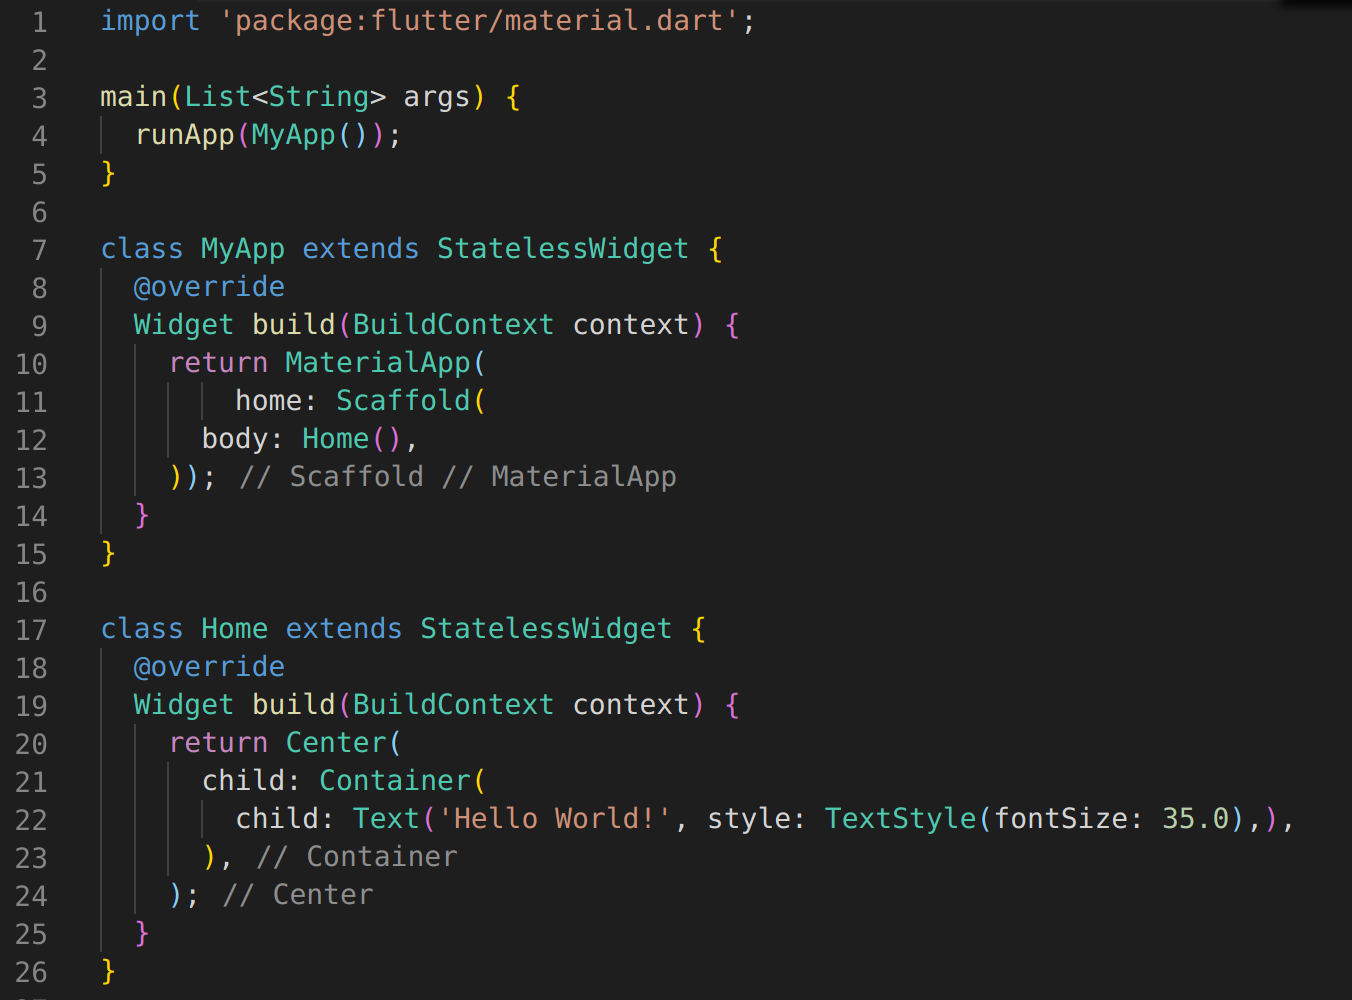
\includegraphics[width=\linewidth, height=7cm]{StateLessApp.png}
			\caption{Esempio di codice di widget stateless}
		\end{subfigure}
		\begin{subfigure}{0.3\linewidth}
			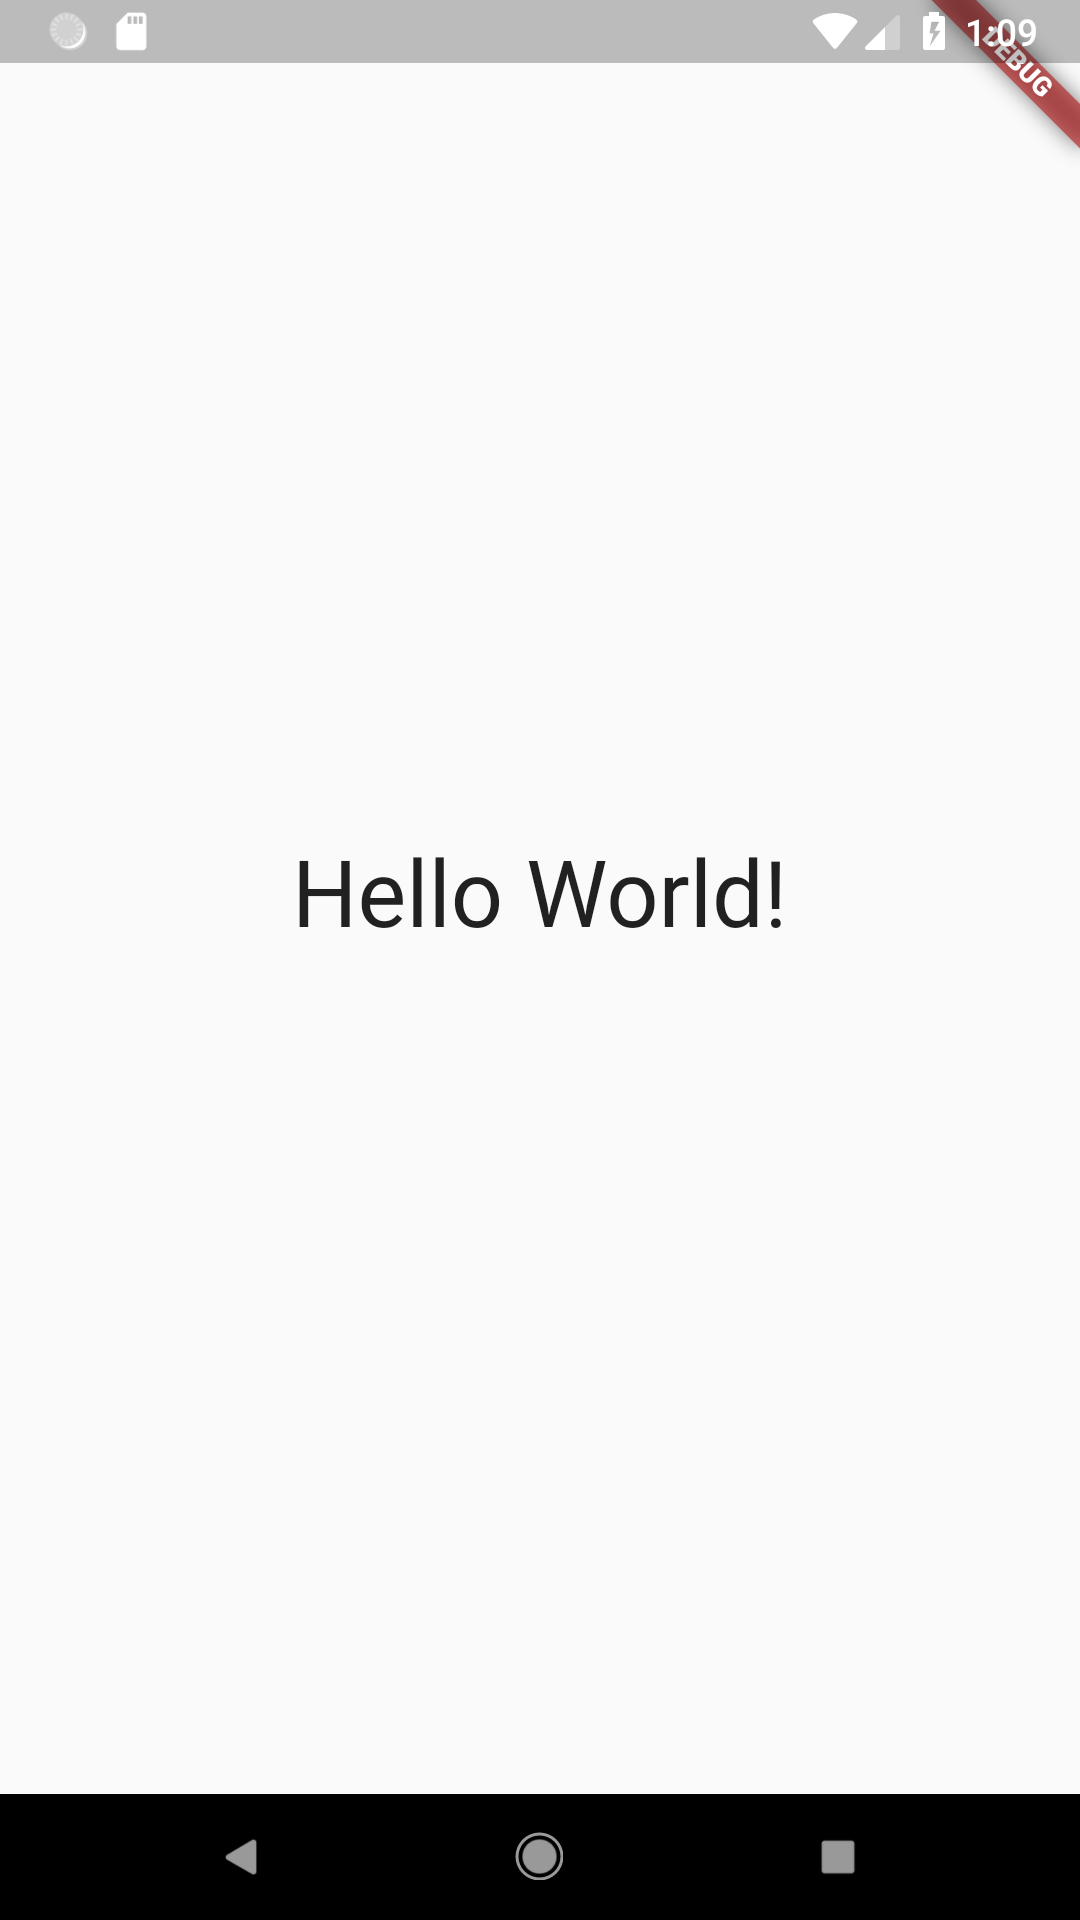
\includegraphics[width=\linewidth, height=7cm]{StateLessScreen.png}
			\caption{Risultato}
		\end{subfigure}
		\caption{}
		\label{stateless1}
	\end{figure} 

	Nell'immagine \ref{statefull} viene mostrato invece un widget di tipo
	Statefull. Si può notare come la prima parte del codice sia identica, con la
	classe MyApp che è ancora un widget senza stato. Ciò che cambia è la classe
	Home che ora è con stato e presenta un unico metodo sovrascritto chiamato
	\textit{createState}. La freccia =$>$ in dart è una notazione per scrivere in
	modo compatto un metodo che ritorna un unico oggetto, in questo caso una
	classe chiamata \_HomeState, che estende State$<$Home$>$. Il trattino basso
	in dart sta a indicare un oggetto privato, a cui quindi non è possibile
	accedere se non in quella specifica classe. \_HomeState possiede una
	varibile di tipo intero denominata counter (anch'essa privata grazie al
	trattino basso) e ha valore iniziale 0. Presenta poi un metodo denominato
	buttonPressed al cui interno risiede una funzione molto importante, la
	\textit{setState}. Quando viene compilata una sezione di codice che sta
	all'interno di tale funzione, viene richiamata la funzione build del widget
	in esecuzione ed è quindi grazie ad essa che l'app diventa interattiva, in
	quanto tramite azioni dell'utente cambiano i valori delle variabili.
	Nell'esempio è presente un pulsante (FloatingActionButton) che aumenta il
	valore della variabile counter, che viene stampato a schermo. Da notare
	infine come si possa accedere al metodo toString di un oggetto in dart
	anteponendo al suo nome il carattere \$.

	\begin{figure}[h!]
		\centering
		\caption{Esempio di codice di widget statefull}{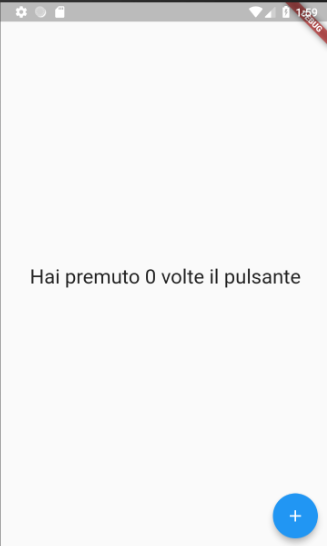
\includegraphics[scale=0.35]{StateFullApp.png}\label{statefull}}
	\end{figure}

	\section{Principali Widget}
	% \subsection{Principali Widget}
	Di seguito vengono riportati i widget di cui si è fatto maggiore uso
	all'interno dell'applicazione.
	
	\begin{trivlist}
		\item \textbf{Text} \newline
		Questo widget permette di mostrare a schermo le stringhe fornite come
		primo argomento al suo costruttore (\verb|Text("Testo da mostrare")|).
		Il testo può svilupparsi su più righe o su una sola a seconda delle
		costanti di layout della particolare schermata nella quale risiede il
		widget. Nel costruttore possono essere indicati diversi argomenti
		opzionali, tra cui lo stile. Se si vuole indicare un particolare stile
		al proprio testo bisogna inserire un TextStyle, cioè un'ulteriore classe
		che gestisce il font, l'inserimento del grassetto o del corsivo e la
		formattazione dell'intero testo (giustificato, allineato a sinistra o a
		destra e centrale).  
		\item \textbf{Row, Column} \newline
		Questi widget vengono spesso utilizzati per ottenere schermate ordinate
		e gradevoli dal punto di vista estetico all'utilizzatore. Il parametro
		principale di entrambe è l'argomento \verb|children| (e non \verb|child| come
		spesso accade per altre classi), proprio perchè sono pensati per
		contenere diversi widget disposti rispettivamente in orizzontale o in
		verticale. La loro grandezza in pixel sarà formata dalla somma della
		dimensioni di ciò che contengono e si possono ancora una volta inserire diverse
		preferenze di stile come la posizione rispetto all'asse principale o
		secondario. Nella figura \ref{rowColumn} si possono vedere i due widget
		che possiedono quattro Container figli di diverso colore.
		\begin{figure}[h!]
			\centering
			\begin{subfigure}{0.3\linewidth}
				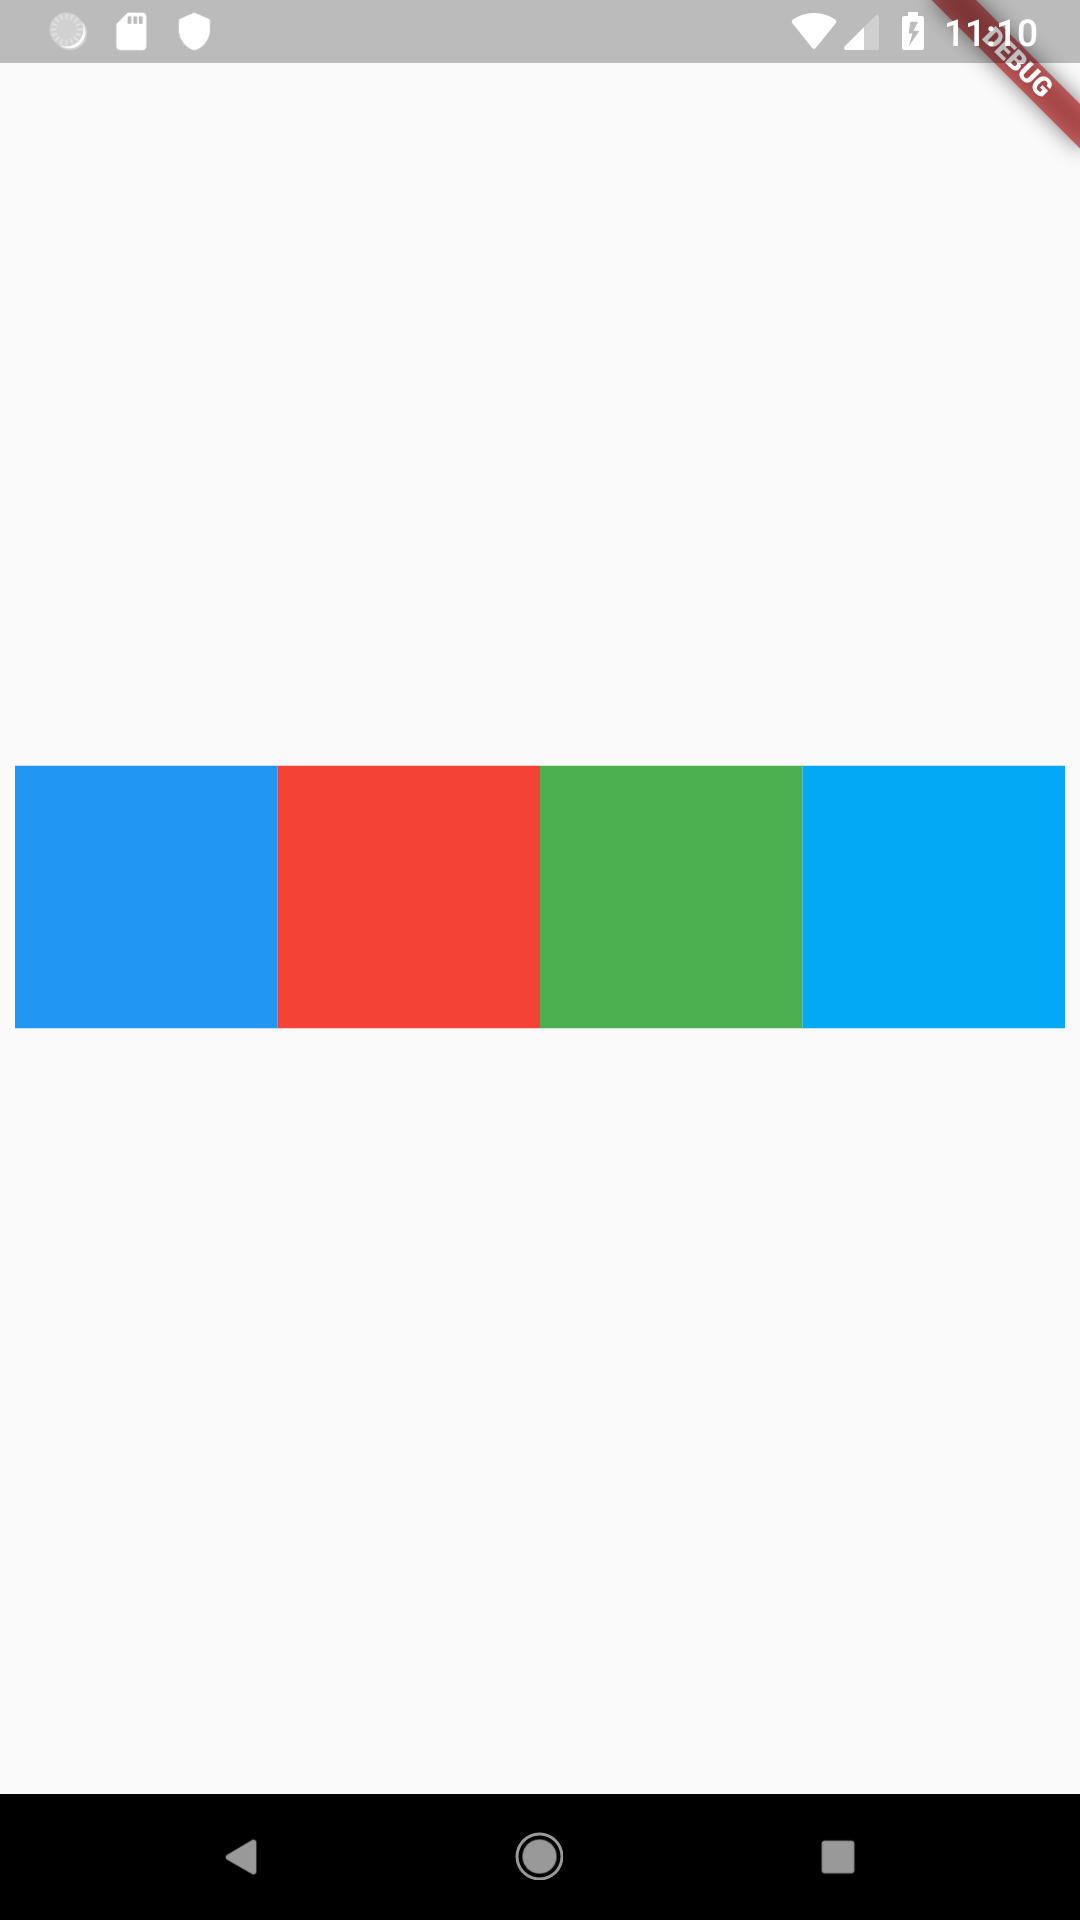
\includegraphics[width=\linewidth]{Row.png}
				\caption{Row}
			\end{subfigure}
			\begin{subfigure}{0.3\linewidth}
				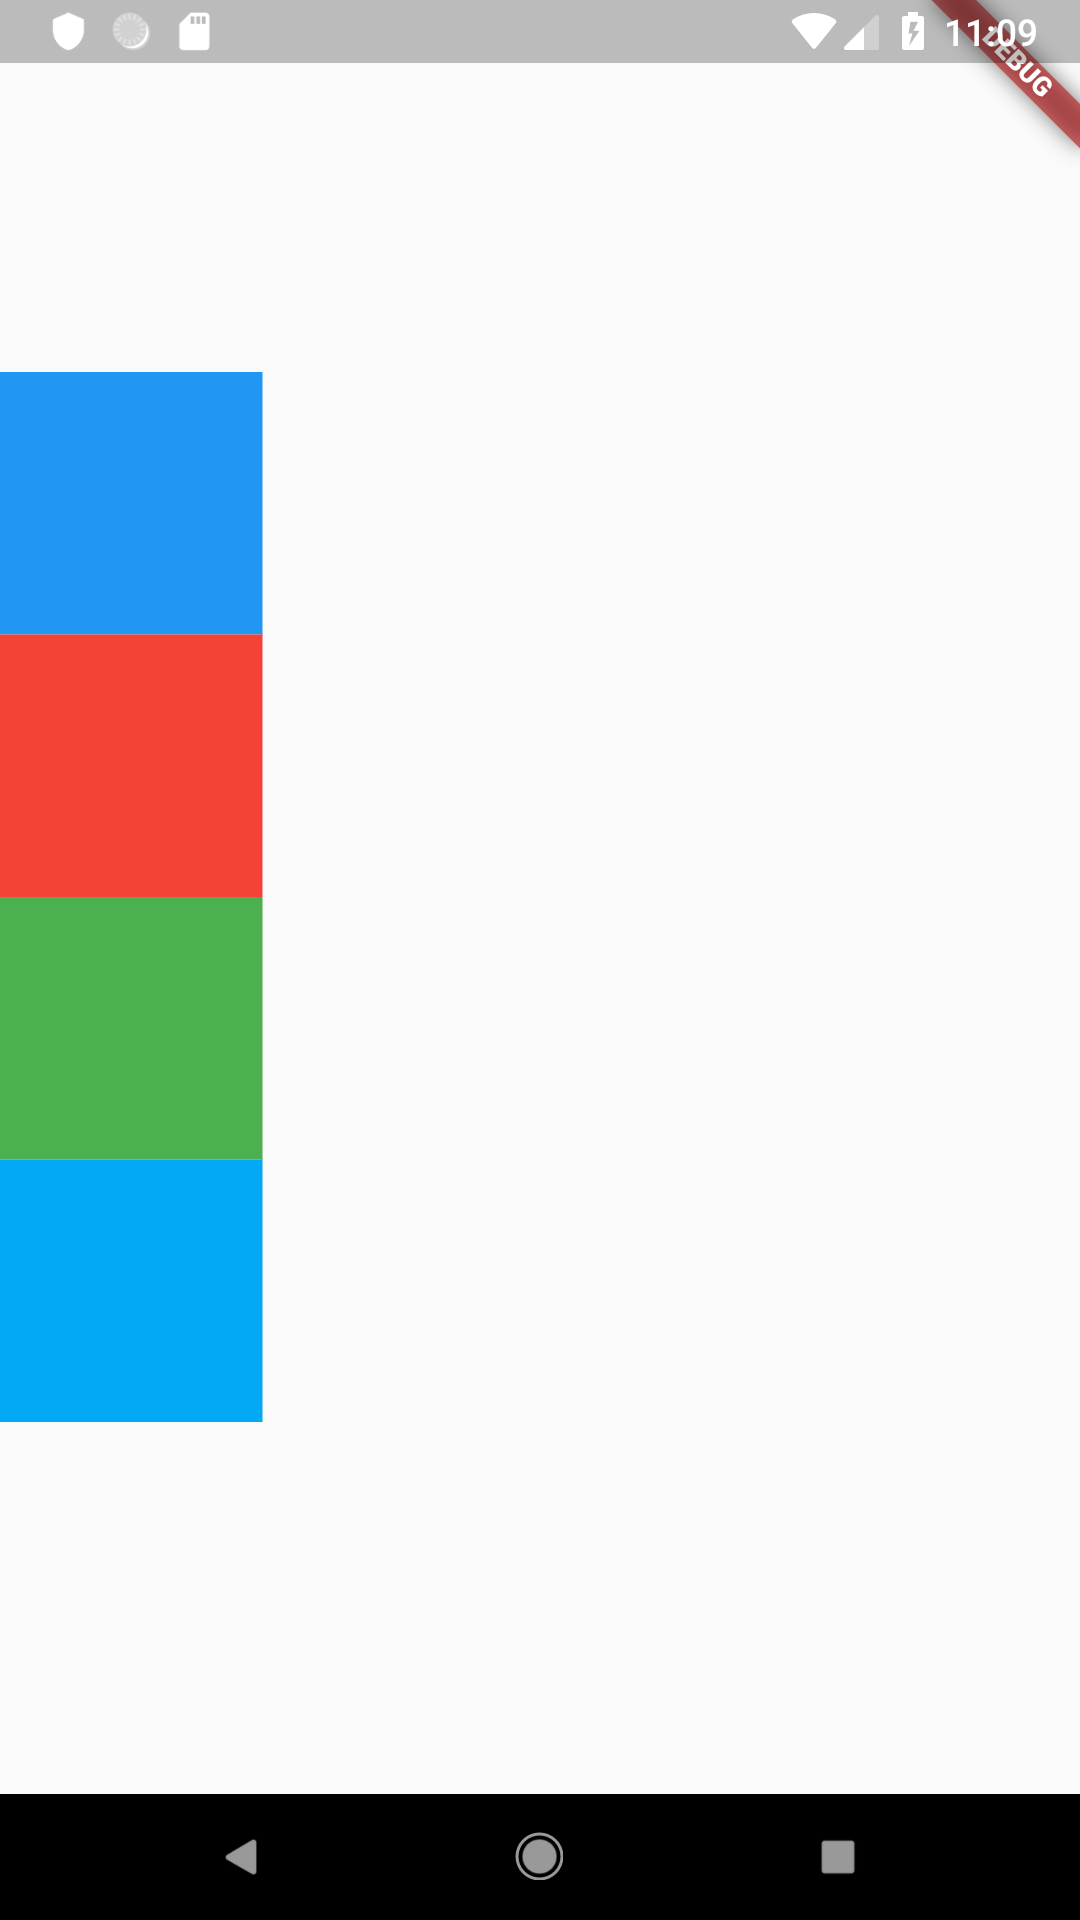
\includegraphics[width=\linewidth]{Column.png}
				\caption{Column}
			\end{subfigure}
			\caption{}
			\label{rowColumn}
		\end{figure} 
		\item \textbf{Stack} \newline
		\'E simile ai due precedenti in quanto anch'esso contiene diversi widget
		figli. Se ne differenzia in quanto non privilegia un'unica direzione di
		posizionamento, ma si può indicare per ogni figlio la posiziona esatta
		in pixel che dovrà avere sullo schermo. Questo passaggio viene
		effettuato racchiudendo il widget che si vuole inserire all'interno di
		un'istanza della classe Positioned (che sarà uno dei figli dello Stack)
		e indicando gli esatti pixel nel suo costruttore. 
		\item \textbf{Container} \newline
		Crea un elemento rettangolare che avrà come altezza e lunghezza le
		minime dimensioni per poter contenere il widget indicato come child. \'E
		molto utilizzato nel momento in cui si vuole migliorare graficamente una
		schermata in quanto tramite il parametro opzionale decoration si può
		introdurre una nuova classe chiamata BoxDecoration che gestisce un
		grande insieme di aspetti grafici come i contorni (angoli e
		ombre) o riempire con un colore o un'immagine il Container.
	\end{trivlist}

	\section{Material Design}
	% \subsection{Material Design}
	Il Material Design è un linguaggio visuale che unisce i classici principi di
	un buon design con l'innovazione della tecnologia e della scienza. 
	\cite{material} \newline
	Tale design è interamente sviluppato da Google e fa uso di layout basati su
	una griglia, animazioni e transizioni. Si prendono ora in cosiderazione i
	widget più comuni appartenenti a questo particolare design.
	\begin{trivlist}
		\item \textbf{Scaffold} \newline
		Implementa la struttura (\textit{impalcatura}) del layout visuale di
		base del material design. Si espande fino a occupare tutto lo spazio
		disponibile sullo schermo, inoltre quando appare una tastiera a seguito
		di un'interazione con l'utente la grandezza di questo widget cambia in
		base alle dimensioni di quest'ultima. Presenta nel proprio costruttore
		argomenti per mostare sulla schermata Drawer, SnackBar e BottomSheets,
		descritte di seguito. 
		\item \textbf{AppBar} \newline
		Un'AppBar consiste in una linea orizzontale, solitamente posizionata in
		alto sulla schermo, che contiene diverse azioni (IconButtons) seguite da
		un menù a comparsa (PopUpMenu). In questo modo si possono inserire in un
		unico luogo tutte le scorciatoie per passare da una schermata ad
		un'altra oppure si possono accorpare funzionalità utili a portata di
		mano per l'utente. Bisogna inserire come argomenti il titolo dell'AppBar
		e inoltre una serie di azioni (\textit{actions}) sottoforma di una lista
		di widget. 
		\begin{figure}
			\centering
			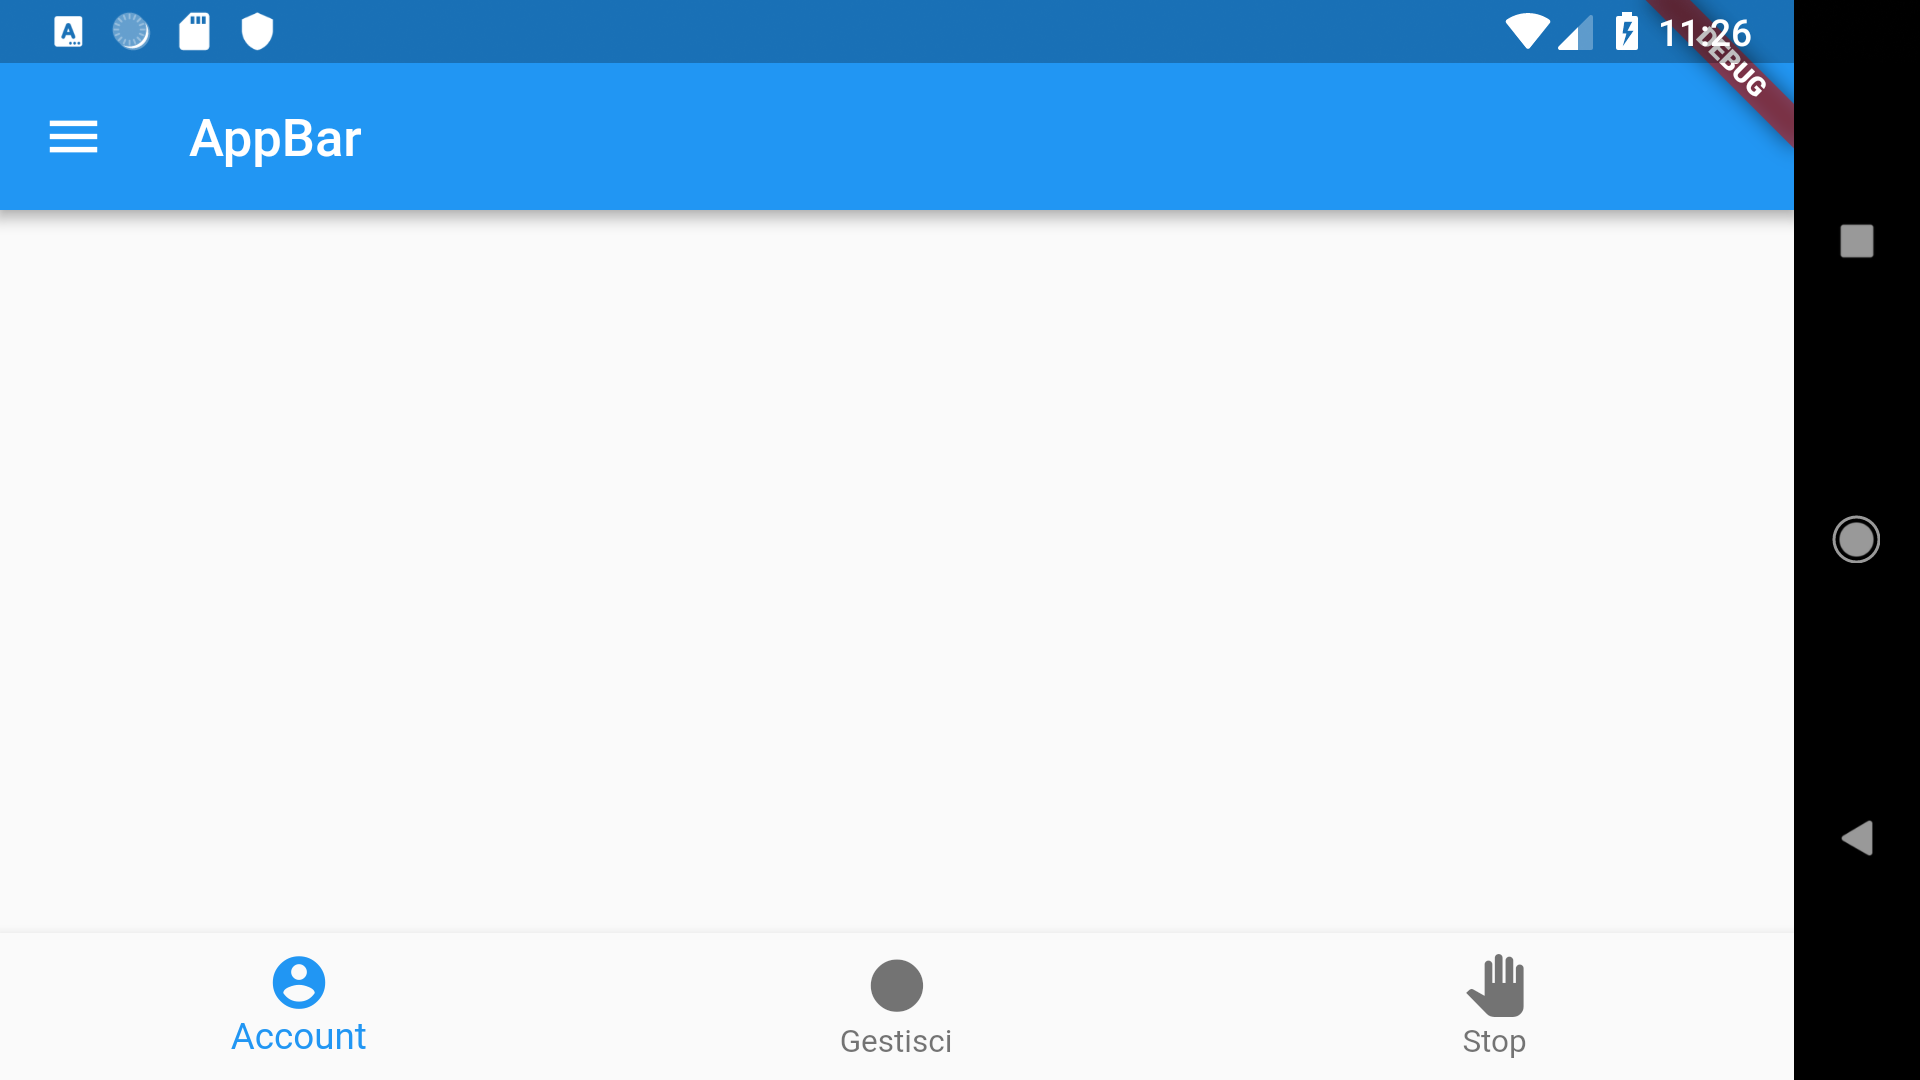
\includegraphics[width=0.9\linewidth]{Scaffold.png}			
			\caption{Nell'esempio viene mostrata una Scaffold, che fa da widget
			genitore all'AppBar posizionata in alto, al Drawer in alto a
			sinistra e alla BottomNavigationBar in basso con tre icone con
			titolo. Si noti inoltre come venga gestita in automatico la
			possibilità di ruotare il proprio dispositivo, cambiando
			l'orientazione della schermata.}
		\end{figure}
		\item \textbf{BottomNavigationBar} \newline
		\'E un material widget disposto in fondo allo schermo per selezionare un
		piccolo numero di schermate, solitamente tra le tre e le cinque.
		Si costruisce tramite diversi strumenti quali widget di testo, icone o
		entrambi. Se gli elementi figli sono minori di quattro, la grandezza di
		ogni item è fissa, mentre se superiore la grandezza si adatta al numero
		di widget contenuti.
		\item \textbf{Drawer} \newline
		Consiste in un pannello che entra in orizzontale sullo schermo
		solitamente dal lato sinistro della Scaffold. Come figlio è solito avere
		una ListView (particolare tipo di Column che gestisce anche lo scroll
		verticale), in modo da mostrare all'utente utili link per la navigazione
		all'interno dell'applicazione. L'AppBar mostra in automatico un Drawer
		vuoto con la classica icona dei menù a comparsa se non viene specificato
		nulla nel suo costruttore.
		\item \textbf{SnackBar} \newline
		Formato da un messaggio con un'azione opzionale visualizzato brevemente
		nella parte inferiore dello schermo, viene utlizzato per comunicare
		all'utente una particolare informazione come l'attesa per un caricamento
		o il manifestarsi di un problema a seguito di un errore, come la
		mancanaza di una connessione internet.
		\item \textbf{FlatButton e IconButton} \newline
		Sono entrambi pulsanti che si differenziano per ciò che contengono. Il
		primo è solitamente formato da un rettangolo (i cui angoli possono
		essere smussati a piacere) al cui interno risiede un testo esplicativo
		dell'azione che verrà eseguita a seguito di un tocco da parte
		dell'utente. Il secondo è invece circolare e contiene un'icona che
		dovrebbe mostrare direttamente quale sarà la sua funzione. Entrambi sono
		widget di tipo Statefull, in quanto il loro colore o la loro forma può
		cambiare a seguito di pressioni sullo schermo.
		\item \textbf{TextField} \newline
		Consente all'utente di inserire del testo, attraverso l'uso della
		tastiera che appare sullo schermo. Il widget chiama la funzione
		\textit{onChanged} ogni volta che viene modificato il testo nel campo. Se
		l'utente indica di aver finito di digitare (ad esempio
		premendo il pulsante di invio), si attiva
		la funzione \textit{onSubmitted}. Per controllare il testo visualizzato nel
		TextField si può utilizzare una particolare classe chiamata
		\verb|TextEditingController|, ad esempio per impostare
		un valore iniziale già presente all'avvio della schermata o per inserire
		i caratteri scritti dall'utente in un'altra variabile.
		\begin{figure}
			\centering
			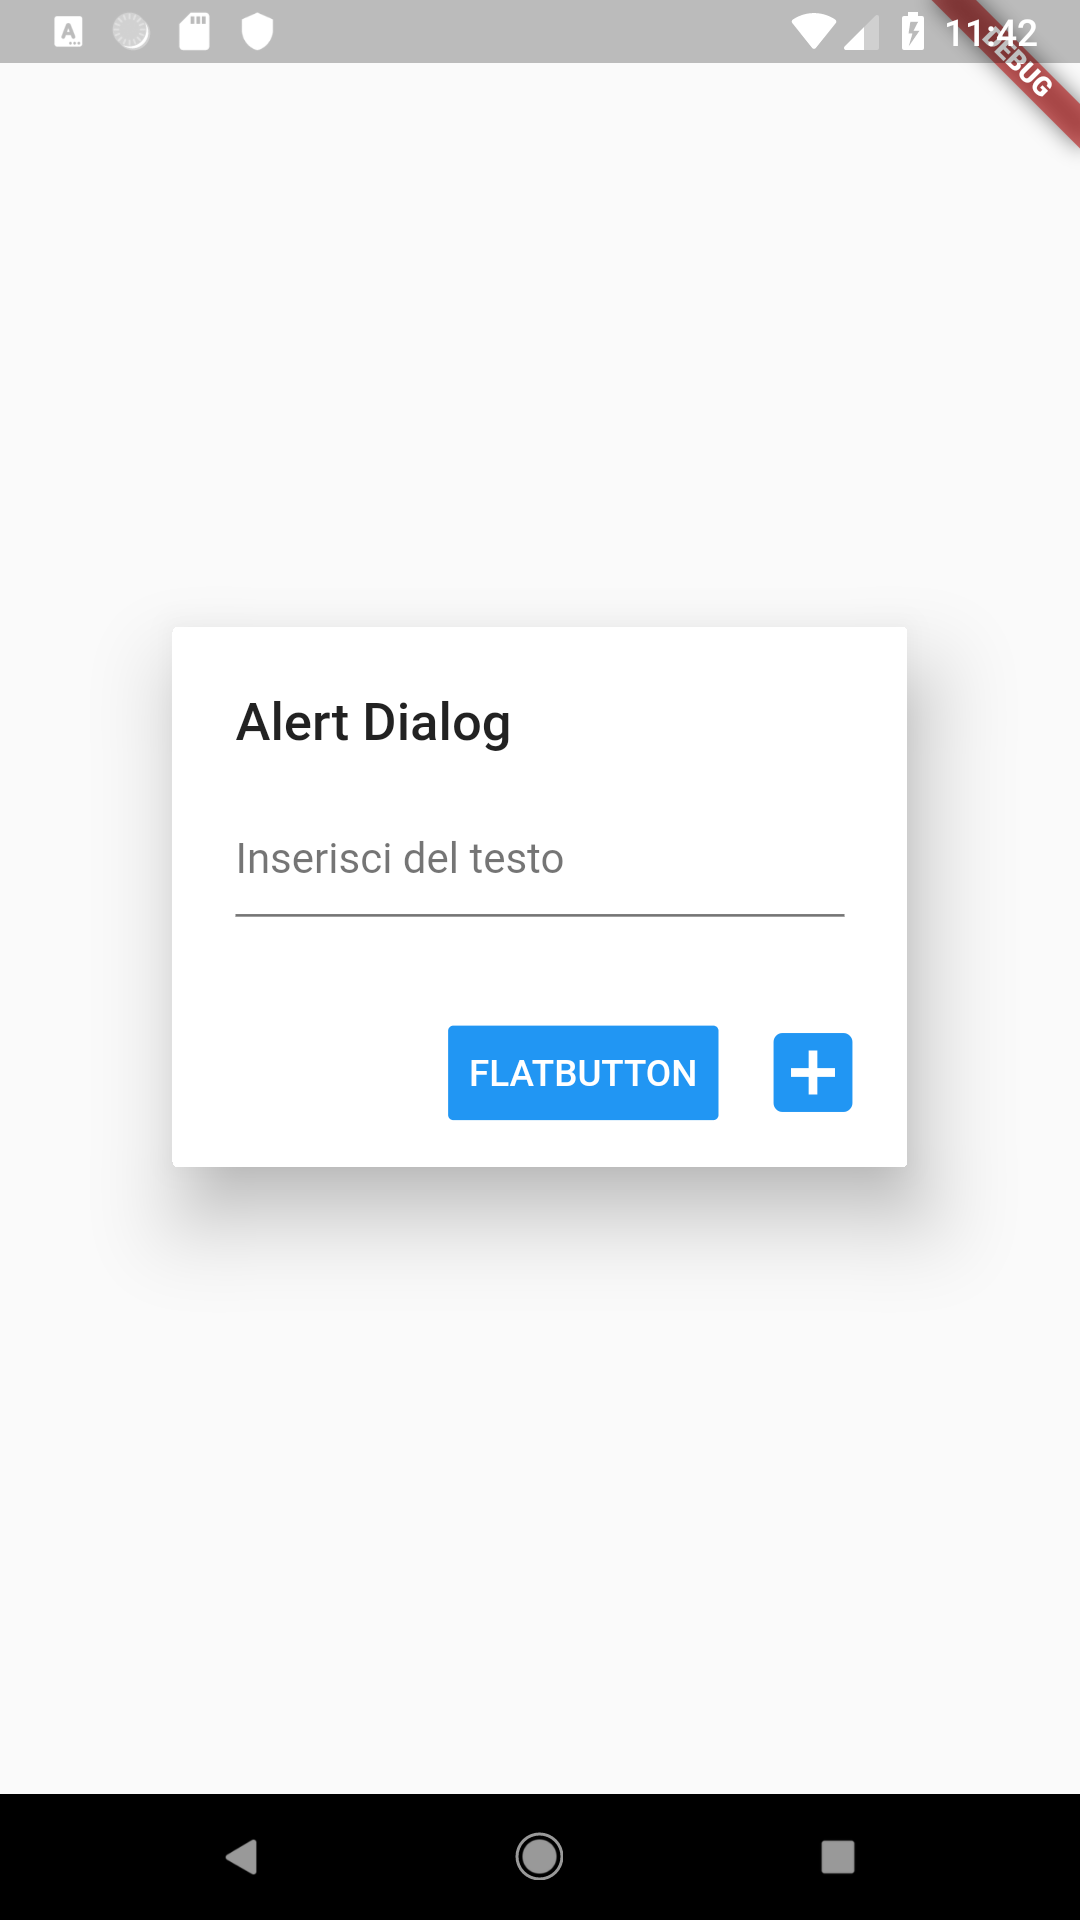
\includegraphics[width=0.4\linewidth]{AlertDialog.png}			
			\caption{Nell'esempio viene mostrata una Scaffold che contiene
			un'AlertDialog. Quest'ultima presenta un titolo, un contenuto
			formato da una TextForm per inserire del testo, e due pulsanti,
			quello a sinistra è un FlatButton mentre quello a destra è un IconButton.}
		\end{figure}
		\item \textbf{AlertDialog} \newline
		Una AlertDialog informa l'utente sulle situazioni che richiedono una
		conferma di un'operazione. Inoltre ha un titolo opzionale e un
		elenco opzionale di azioni. Il titolo viene visualizzato in alto e le
		azioni vengono visualizzate sotto il contenuto dell’AlertDialog. Si può
		anche scegliere che se l'utente tocca al di fuori dell'area dedicata a
		questo widget esso sparisca, oppure si può decidere che l'AlertDialog si
		dissolva solo a seguito della pressione di un particolare tasto.
		\item \textbf{BottomSheet} \newline
		Il BottomSheet è un particolare widget che appare nella parte inferiore
		dello schermo e occupa spazio in base alla grandezza del proprio figlio
		(solitamente una Column o una ListView). Esistono due tipologie: fisso e
		dinamico. La prima rimane visibile anche quando l'utente interagisce con
		altre parti dell'app. Può essere creato e visualizzato  con
		la funzione \textit{ScaffoldState.showBottomSheet}. La seconda tipologia
		è un'alternativa a un menù o a una AlertDialog e impedisce all'utente di
		interagire con il resto dell'app. I BottomSheet di questo tipo possono
		essere creati e visualizzati con
		la funzione \textit{showModalBottomSheet}.
	\end{trivlist}

	\section{Animation}
	% \subsection{Animation}
	Le Animation rendono l'interfaccia più intuitiva, contribuiscono a
	rendere elegante 
	l'aspetto di un'app e migliorano l'esperienza dell'utente. Il
	supporto di Flutter semplifica l'implementazione di una grande varietà di tipi di
	animazioni. Molti widget, in particolare i Material Widget, hanno
	animazioni standard definite nelle loro specifiche di progettazione, 
	anche se il programmatore può crearne di nuove personalizzando quelle già esistenti. \\
	Sono implementati due tipi di animazioni: Tween e Physic-based. Nella prima tipologia
	(che è l'abbreviazione di \textit{in-betweening}, traducibile come "nel frattempo,
	in mezzo"), vengono definiti l'aspetto e la forma iniziali e finali del
	widget, insieme alla durata e alla velocità dell'animazione. Il framework
	calcola poi automaticamente come effettuare la transizione in base ai dati
	che vengono forniti al costruttore della particolare Animation. La seconda
	tipologia cerca invece di gestire quegli elementi che vogliono rappresentare
	comportamenti del mondo reale, cercando di modellare i movimenti e le
	dinamiche di oggetti concreti. Per esempio per muovere una piccola sfera la
	velocità con cui essa rimbalzerà dipenderà dalla spinta iniziale che le è
	stata posta mentre l'altezza del salto dipenderà invece da quanto essa sia lontana dal terreno.
	Nello specifico esiste una classe chiamata AnimationController che possiede
	il metodo \textit{animateWith} e inoltre è possibile simulare il
	comportamento di una molla con la classe SpringSimulator.
	


	
